The mean cumulative function (MCF) is often the focus in a nonparametric
analysis of recurrent data. Let \(M_i(t)=\mathbb{E}\{N_i(t)\}\) denote
the MCF of \(N_i(t)\). The Nelson-Aalen estimator \citep{nelson2003siam}
are widely utilized in exploring the trend of recurrent event data.
\[\hat{M}(t) = \int_0^t \frac{dN(s)}{\delta(s)},\] where
\(dN(s)=\sum_{i=1}^k dN_i(s)\),
\(\delta(s) = \sum_{i=1}^k \delta_i(s)\), \(dN_i(s)\) and
\(\delta_i(s)\) is, respectively, the jump size and at-risk indicator of
process \(i\) at time \(s\).

We may use the \texttt{mcf()} function and the associated
\texttt{plot()} method provided by the \pkg{reda} package to visualize
MCF estimates stratified by whether the patients receive chemotherapy as
follows. Terminal events are ignored here for ease of illustration.

\begin{Shaded}
\begin{Highlighting}[]
\NormalTok{re_mcf <-}\StringTok{ }\KeywordTok{mcf}\NormalTok{(}\KeywordTok{Recur}\NormalTok{(t.stop, id, event) ~}\StringTok{ }\NormalTok{chemo, }\DataTypeTok{data =} \NormalTok{df0)}
\KeywordTok{plot}\NormalTok{(re_mcf, }\DataTypeTok{conf.int =} \OtherTok{TRUE}\NormalTok{, }\DataTypeTok{lty =} \DecValTok{1}\NormalTok{:}\DecValTok{2}\NormalTok{) +}
\StringTok{    }\NormalTok{ggplot2::}\KeywordTok{theme}\NormalTok{(}\DataTypeTok{legend.position =} \StringTok{"bottom"}\NormalTok{)}
\end{Highlighting}
\end{Shaded}

\begin{figure}[H]
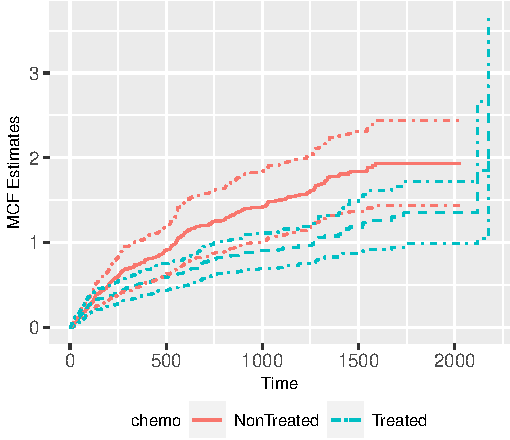
\includegraphics[scale = 1]{reda-mcf_files/figure-latex/plot-sampleMcf-1}
\end{figure}

Furthermore, we may compare the MCF estimates using pseudo-score tests
\citep{cook1996biometrics} as follows:

\begin{Shaded}
\begin{Highlighting}[]
\KeywordTok{mcfDiff.test}\NormalTok{(re_mcf)}
\end{Highlighting}
\end{Shaded}

\begin{verbatim}
Two-Sample Pseudo-Score Tests:
                Statistic Variance  Chisq DF Pr(>Chisq)  
Constant Weight     47.49   416.71   5.41  1      0.020 *
Linear Weight       36.56   263.59   5.07  1      0.024 *
---
Signif. codes:  
0 '***' 0.001 '**' 0.01 '*' 0.05 '.' 0.1 ' ' 1

Variance Estimator: robust 
\end{verbatim}
